\chapter{自动加样系统软件设计方案的确定}

\section{加样系统程序结构设计}
根据本文设计的自动加样系统功能动作分析可知,程序上电后,执行加样命令,机械臂动作,这里,X(水平)方向的运动由步进电机驱动滚珠丝杠,丝杠驱动同步带完成;Y(垂直)方向的运动同理。注射泵取样和释样原理:步进电机驱动丝杆运动,丝杆进而带动螺母推动活塞移动进行取样和释样。加样针移动至待检试剂液瓶液面上方,液面检测方式采用电容式液面检测装置,检测到液面位置时取样针下降至液面一下3$mm$进行取样。(2)取样动作完成后,取样针移动至试剂反应瓶液面上方,同样进行液面检测,检测到液面后下降至液面以下3$mm$进行释放样液。(3)释样动作完成后,加样针移动至清洗池进行清洗。(4)清洗动作完成后,加样针在加样机械臂带动下复位,复位动作完成后即进行完一个加样周期,等待下一个加样命令。系统程序结构流程图如\ref{fig:6-1}

\begin{figure}[htbp!]
	\centering
	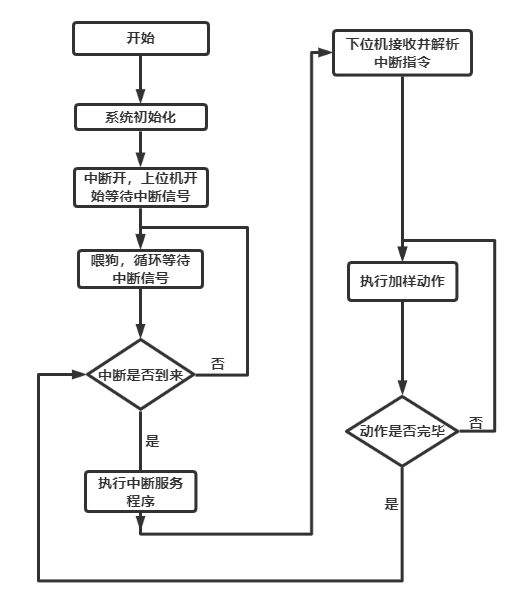
\includegraphics[height=11.5cm]{chap/figure/6-1.jpg}
	\caption{主程序结构流程图}
	\label{fig:6-1}
\end{figure}